% !TEX root = ../TechProject.tex

\graphicspath{{Chapter5/}}


\chapter{Experiment}


This part will answer the research question: 
\\
\\
\textit{Is the proposed method a suitable solution to automate recommendations of songs suitable for adding to a given DJ set?}.
\\
\\
As explained in the hypothesis. I'm testing a music recommendation system that uses MixesDB as a dataset and see whether it garners appropriate results.

The idea for the testing came from the million playlist dataset from Spotify \citep{aicrowd_aicrowd_2023}.  Where they both had the dataset (million untouched Spotify playlists) and the challenge dataset, which contained many modified playlists, showing how many missing songs are in each playlists.

As the dataset utilized was obtained from mixesDB, it was necessary to devise a customized approach for the preparation of the evaluation set.

\subsection{Preparing Evaluation Set}
During the evaluation phase of the study conducted on the million playlist dataset, the quality of a given applications trained on this dataset was assessed through a range of methods that involved analysing both missing and recommended songs. In order to effectively compare different applications, it was essential to create a standardised evaluation set that incorporated aspects of the Spotify data set, which could show the applications that can recommend songs that were featured in the playlists originally.

\begin{figure}[H]
	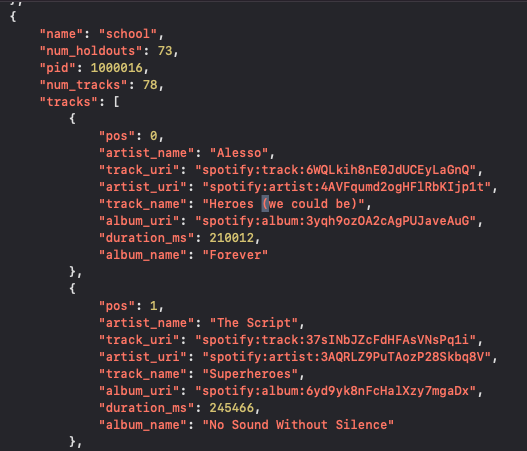
\includegraphics[scale=0.5]{images/spotify_challenge_set}
	\centering
	\caption{Screenshot of spotify challenge set. \citep{aicrowd_aicrowd_2023}} 
\end{figure}

The Spotify challenge set consisted of 10,000 playlists with varying numbers of input songs, ranging from 0 to 100 tracks. For each of these playlists, Spotify requested 500 track recommendations from the participating teams \citep{aicrowd_aicrowd_2023}. However, due to the relatively smaller scale of the dataset and difference between playlists and DJ sets under consideration, various aspects of this challenge set had to be downscaled to maintain the academic rigour of the study. For instance, the range of input songs was considerably narrower, as DJ sets typically have a minimum length of 10 tracks, compared to playlists that can have varying lengths.

To ensure the feasibility of finding all songs in the evaluation set, an additional criterion was applied, whereby each song had to have a total play count of at least 5. Furthermore, the input and missing songs were divided in a standardized manner, with 20\% of the songs allocated as missing songs, and the remaining 80\% as input songs. Overall, the creation of the evaluation set was a crucial aspect of the study, ensuring that the assessment of the applications was based on a consistent and standardized evaluation framework.

\begin{figure}[H]
	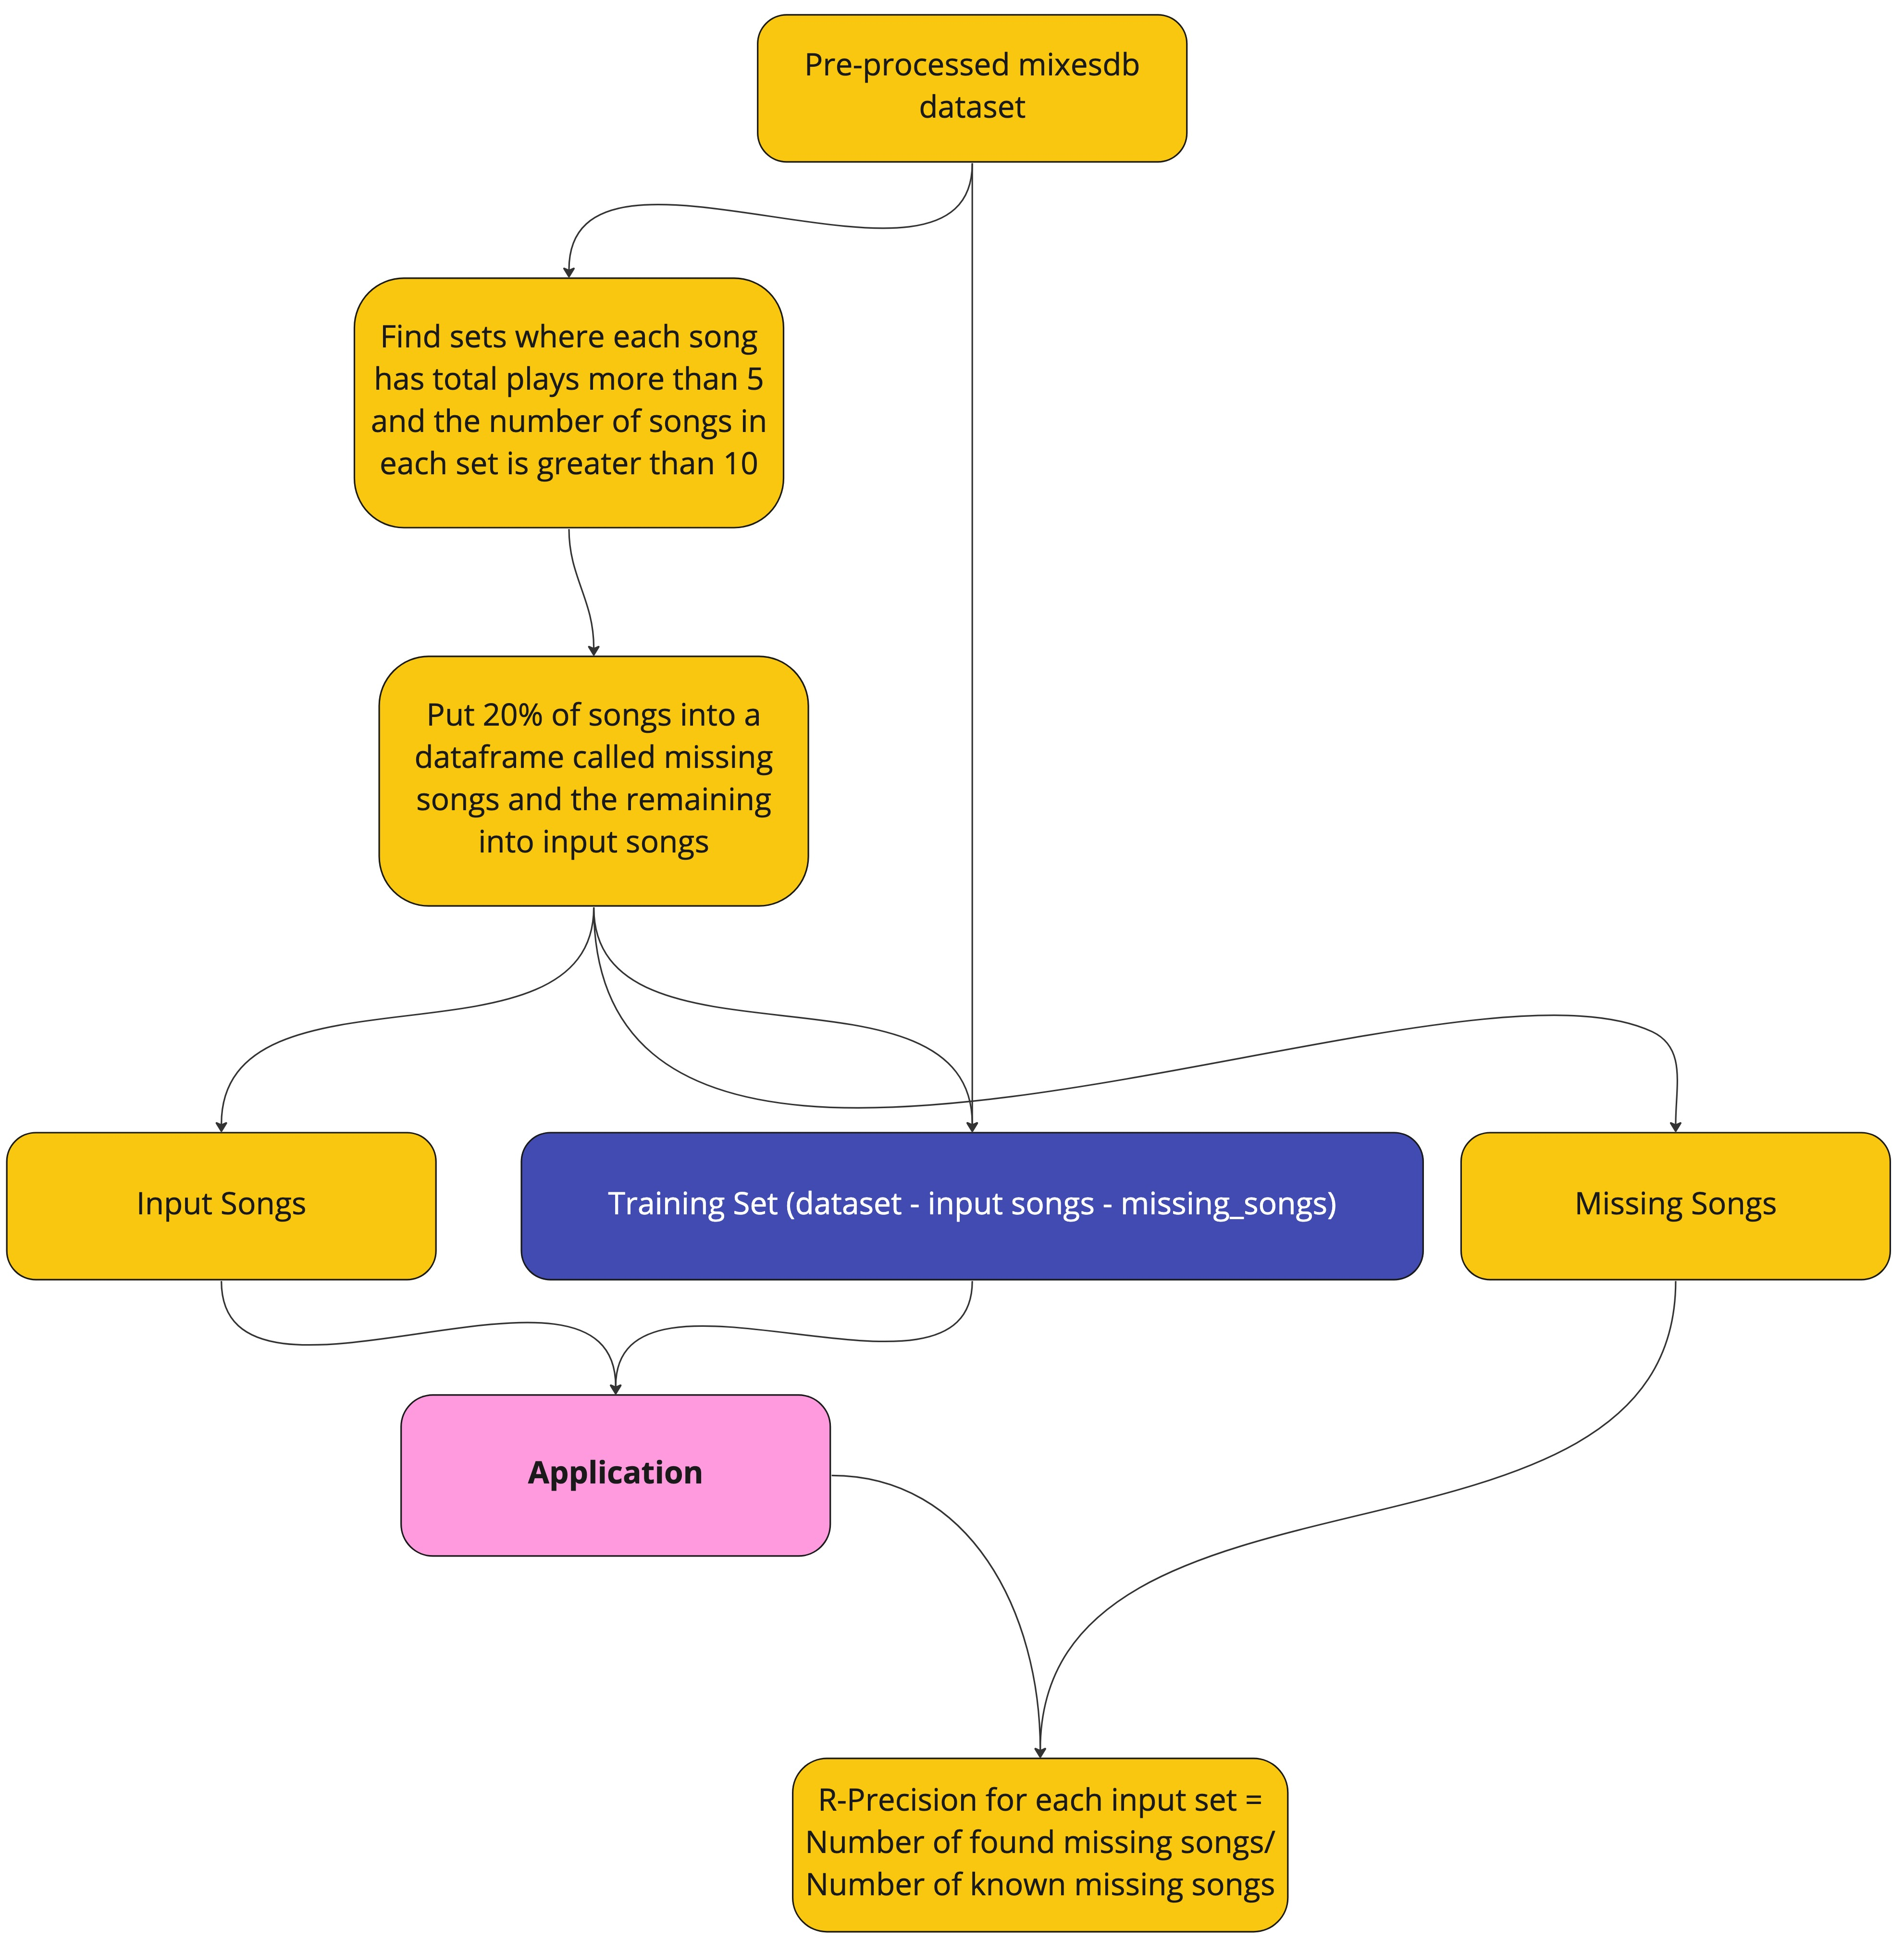
\includegraphics[scale=0.1]{images/evaluation_set_app_flow}
	\centering
	\caption{Application flow of the creation of the evaluation set} 
\end{figure}


\subsection{R-Precision}
The first mean of testing would be finding the R-precision. The R-precision is the amount of found tracks that were originally in the mix divided by the number of known missing tracks.

\begin{equation}
	R-Precision = \frac{|G\cap R_{1:|G|}|}{|G|}
\end{equation}

The average R-Precision got tested on varying latent factor values, and when the highest is found, we alter the amount of songs in the input, to see what size an input gets the best results.


